\Section{Code Malleability: A Case Study}
\label{section:chroma}

A contrast of chroma format support between the StreamIt and  C
reference implementations illustrates the benefits stream based
languages can  provide to programmability. While the conceptual
difference between chroma formats is merely a change in
downsampling ratio, this leads to a change in the data rates and the
ratios of data between the color channels. This requires that the C
implementation parameterize its buffer sizes, array lengths, array
indices, and pointer offsets on the chroma format; the reference
implementation uses a  ``chroma flag'' to dictate control flow to
alternate index/offset calculations  in 43 locations in the code. As
an example, a fragment of the ``form\_prediction'' routine  (in
recon.c~\cite{reference-mpeg-c}) used for motion compensation is shown
in  Figure~\ref{fig:chroma}. This function calls a  subroutine to
perform the actual motion compensation on each of the three color
channels, passing in array offsets to a global array holding the
data. Lines 4-6 adjusts values used for address calculations to handle
the 4:2:2 and 4:2:0 chroma formats, and lines 7-9 provide
additional adjustments for the 4:2:0 format. While these offset
adjustments are neccesary for high performance, they are difficult for
programmers  and make the code hard to understand.

To add support for the 4:2:2 chroma format in our StreamIt decoder, we
modified 31 lines and added 20 new lines. Of the 31 modified lines, 23
were trivial modifications to pass a variable representing the
chroma format as a stream parameter. The greatest substantial
change was to the color channel splitter, previously illustrated on line 20 of 
Figure~\ref{fig:dec_block_detailed}. In the case of a 4:2:2 sampling rate,
the chrominance data, as it appears on the input tape, alternates
between each of the two chrominance channels. Thus, a two-tiered
splitjoin is used to properly recover the appropriate chrominance
channels. The new splitjoin is shown in Figure~\ref{fig:chroma}. 
Even after these modifications, the chroma formmat only explicitly dictates
control flow in 9 locations. Of course, the stream graph execution changes 
dramatically between chroma formats, but these changes will be to 
scheduling and buffer management, which are implicit changes hidden from 
the programmer. 

\begin{figure*}[t]
 \begin{minipage}[t]{4.3in}
   {
    \begin{scriptsize}
    \begin{verbatim}
   // Matt's note - this is the C reference code I added.
   // I added the line numbers so I can reference them in the text.
1    /* Y */
2    form_component_prediction(src[0]+(sfield?lx2>>1:0),dst[0]+(dfield?lx2>>1:0),
3                              lx,lx2,w,h,x,y,dx,dy,average_flag);
4    if (chroma_format!=CHROMA444)  {
5        lx>>=1; lx2>>=1; w>>=1; x>>=1; dx/=2;
6    }
7    if (chroma_format==CHROMA420)  {
8        h>>=1; y>>=1; dy/=2;
9    }
10   /* Cb */
11   form_component_prediction(src[1]+(sfield?lx2>>1:0),dst[1]+(dfield?lx2>>1:0),
12                             lx,lx2,w,h,x,y,dx,dy,average_flag);
13   /* Cr */
14   form_component_prediction(src[2]+(sfield?lx2>>1:0),dst[2]+(dfield?lx2>>1:0),
15                             lx,lx2,w,h,x,y,dx,dy,average_flag);    
    \end{verbatim}
    \end{scriptsize}
   }
   % \vspace{-3pt}
   % \caption{Decoding stream to handle 4:2:0 and 4:2:2 chroma formats.}
   % \label{fig:chroma-stream}
  \end{minipage}
    ~~\hrule~~
 \begin{minipage}[t]{4.3in}
   {
    \begin{scriptsize}
    \begin{verbatim}
    // C = blocks per chrominance channel per macroblock 
    // C = 1 for 4:2:0, C = 2 for 4:2:2
    add splitjoin {
      split roundrobin(4*(B+V), 2*C*(B+V));
      add MotionCompensation() to PT1;
      add splitjoin {
        split roundrobin(N, N);
        for (int i = 0; i < 2; i++) {
          add MotionCompensation() to PT1;
          add ChannelUpsample(C);
        }
        join roundrobin(1, 1);
      }
      join roundrobin(1, 1, 1);
    }
    \end{verbatim}
    \end{scriptsize}
   }
   % \vspace{-3pt}
   % \caption{Decoding stream to handle 4:2:0 and 4:2:2 chroma formats.}
   % \label{fig:chroma-stream}
  \end{minipage}
  ~~\vrule~~
  \begin{minipage}[t]{2.0in}
  {
   \begin{center}
    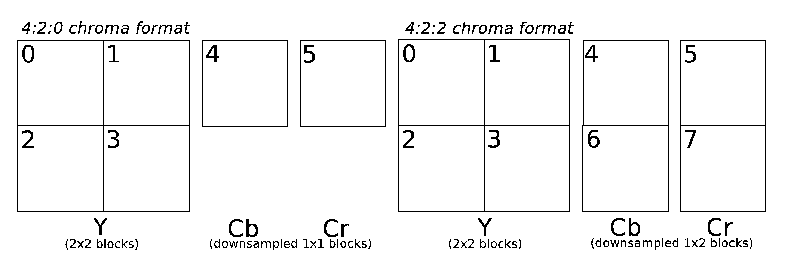
\epsfig{file=chroma_format.eps, width=2.5in}
    % \caption{4:2:0 and 4:2:2 chroma formats showing macroblock ordering}
    % \label{fig:chroma-format}
   \end{center}
  }
  \end{minipage}
  \caption{Decoding stream to handle 4:2:0 and 4:2:2 chroma
    formats. Figures on right illustrate how macroblock orderings
    differ.}
  \label{fig:chroma}
\end{figure*}